
\chapter[Dạng bài: Phương trình vận tốc và phương trình gia tốc trong dao động điều hòa]{Dạng bài: Phương trình vận tốc và phương trình gia tốc trong dao động điều hòa}
\section{Lý thuyết}
\subsection{Vận tốc trong dao động điều hòa}
\subsubsection{Phương trình vận tốc trong dao động điều hòa}
Vận tốc là đạo hàm của li độ theo thời gian:
\begin{equation*} 
	v=x'=-\omega A \sin (\omega t +\varphi)=v_\text{max}\cos \left( \omega t+\varphi+\dfrac{\pi}{2}\right), 
\end{equation*}
trong đó, $v_\text{max}=\omega A$ là vận tốc cực đại.

\subsubsection{Đặc điểm vận tốc trong dao động điều hòa}
\begin{itemize}
	\item Ở vị trí biên ($x=\pm A$) thì vận tốc \bltext{bằng 0};
	\item Ở vị trí cân bằng ($x=0$) thì vận tốc \bltext{có độ lớn cực đại} ($v_{\text{max}} = \omega A$).
\end{itemize}
\subsection{Gia tốc trong dao động điều hòa}
\subsubsection{Phương trình gia tốc trong dao động điều hòa}
Gia tốc là đạo hàm của vận tốc theo thời gian:
\begin{equation*} 
	a=v'=-\omega^2 A \cos (\omega t +\varphi) =a_\text{max}\cos \left( \omega t+\varphi+\pi\right), 
\end{equation*}
trong đó, $a_\text{max}=\omega^2 A$ là gia tốc cực đại.

\subsubsection{Đặc điểm gia tốc trong dao động điều hòa}
\begin{itemize}
	\item Ở vị trí cân bằng ($x=0$) thì \bltext{$a=0$};
	\item Vectơ gia tốc luôn hướng về \bltext{vị trí cân bằng} và có độ lớn tỉ lệ với độ lớn của li độ.
\end{itemize}

\subsubsection{Mối liên hệ giữa gia tốc và li độ}
\begin{equation*} 
	a=-\omega^2 x,
\end{equation*}

trong đó $x$ là li độ và $a$ là gia tốc.
\begin{center}
	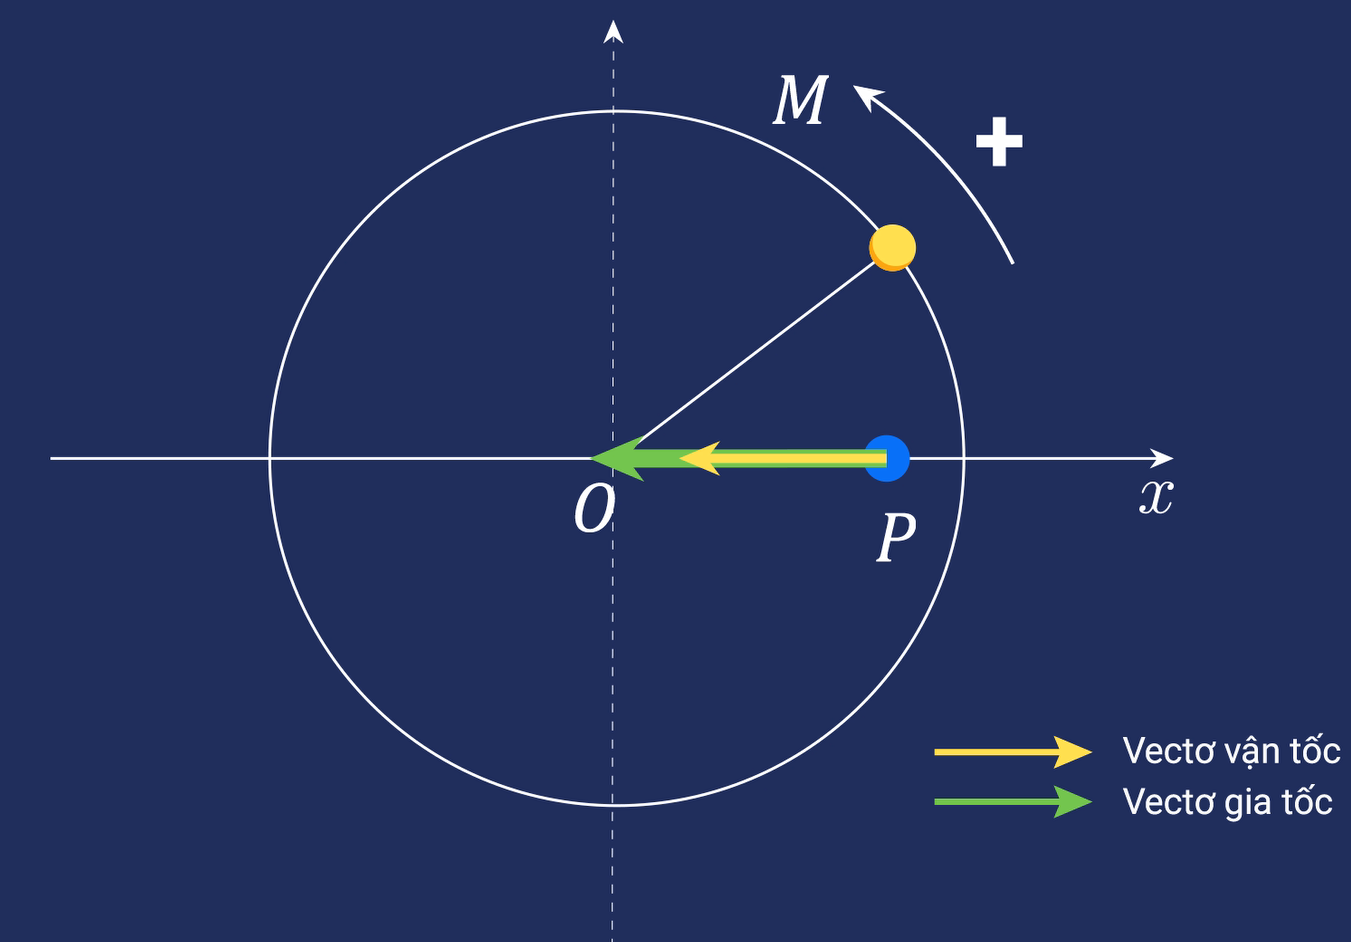
\includegraphics[scale=0.4]{../figs/VN12-PH-02-A-001-2-V2-1.png}
\end{center}
\section{Mục tiêu bài học - Ví dụ minh họa}
\begin{dang}{Giải thích được các đại lượng\\ có trong phương trình vận tốc và gia tốc của vật dao động điều hòa}
	\viduii{2}{Trong dao động điều hòa, vận tốc biến đổi
		\begin{mcq}(2)
			\item cùng pha so với li độ.
			\item ngược pha so với li độ.
			\item sớm pha $\pi / 2$ so với li độ.
			\item trễ pha $\pi / 2$ so với li độ.
		\end{mcq}
	}
	{\begin{center}
			\textbf{Hướng dẫn giải}
		\end{center}
		
		Phương trình tổng quát của vận tốc trong dao động điều hòa là $$v=v_\text{max}\cos \left( \omega t+\varphi+\dfrac{\pi}{2}\right)$$
		
		Do đó vận tốc biến đổi sớm pha $\pi / 2$ so với li độ.
		
		\textbf{Đáp án: C.}
	}
	\viduii{2}{Trong dao động điều hòa, gia tốc biến đổi
		\begin{mcq}(2)
			\item cùng pha so với li độ.
			\item ngược pha so với vận tốc.
			\item sớm pha $\pi / 2$ so với li độ.
			\item sớm pha $\pi / 2$ so với vận tốc.
		\end{mcq}
	}
	{\begin{center}
			\textbf{Hướng dẫn giải}
		\end{center}
		
		Phương trình tổng quát của vận tốc trong dao động điều hòa là $$v=v_\text{max}\cos \left( \omega t+\varphi+\dfrac{\pi}{2}\right)$$
		Phương trình tổng quát của gia tốc trong dao động điều hòa là $$a=a_\text{max}\cos \left( \omega t+\varphi+ \pi\right)$$
		
		Do đó gia tốc biến đổi sớm pha $\pi / 2$ so với vận tốc.
		
		\textbf{Đáp án: D.}
	}
	
\end{dang}
\begin{dang}{Xây dựng được phương trình vận tốc và gia tốc của vật dao động điều hòa}
	\viduii{3}{Một chất điểm dao động điều hòa với phương trình $x=\cos(2\pi t + \pi /6)\ \text{cm}$. Lấy $\pi^2=10$. Biểu thức gia tốc tức thời của chất điểm là
		\begin{mcq}(2)
			\item $a=-2\pi \cos (2\pi t + \pi /6)\ \text{cm/s}^2$.
			\item $a=40 \sin (2\pi t + \pi /6)\ \text{cm/s}^2$.
			\item $a=-40 \cos(2\pi t + \pi /6) \ \text{cm/s}^2$.
			\item $a=2\pi \sin (2\pi t + \pi /6)\ \text{cm/s}^2$.
		\end{mcq}
		
	}
	{\begin{center}
			\textbf{Hướng dẫn giải}
		\end{center}
		Nhận thấy $\varphi$ của cả 4 đáp án đều là $\pi /6$ nên ta áp dụng phương trình gia tốc sao cho $\varphi$ được giữ nguyên:
		$$a=-\omega ^2 A \cos (\omega t + \varphi)$$
		Suy ra $a=-(2\pi)^2 \cos (2\pi t + \pi /6) = -40 \cos(2\pi t + \pi /6) \ \text{cm/s}^2$.
		
		\textbf{Đáp án: C.}
	}
	
	\viduii{2}{Đồ thị vận tốc theo thời gian của một vật dao động điều hòa như hình dưới. Xác định phương trình dao động của vật.
		\begin{center}
			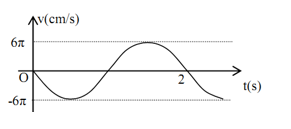
\includegraphics[scale=1]{../figs/VN12-PH-02-A-001-2-V2-2.png}
		\end{center}
		\begin{mcq}(2)
			\item $x=6\cos(\pi t + \pi /2)\ \text{cm}$.
			\item $x=6\cos(\pi t)\ \text{cm}$.
			\item $x=6\cos(\pi t - \pi /2)\ \text{cm}$.
			\item $x=6\sin(\pi t)\ \text{cm}$.
		\end{mcq}
		
	}
	{\begin{center}
			\textbf{Hướng dẫn giải}
		\end{center}
		Tần số góc: $\omega = \dfrac{2\pi}{2}=\pi\ \text{rad/s}$.
		
		
		Dựa vào đồ thị, phương trình vận tốc của vật là
		$$v= 6\pi \cos(\pi t + \pi /2)\ \text{cm/s}$$
		Mà theo công thức: $v=v_\text{max}\cos(\omega t + \varphi + \pi /2)$, suy ra phương trình dao động là
		$$x=A\cos (\omega t + \varphi) = \dfrac{6\pi}{\pi}\cos (\pi t + \pi /2 - \pi /2) = 6\cos(\pi t)\ \text{cm}$$
		
		\textbf{Đáp án: B.}
	}
\end{dang}
\begin{dang}{Sử dụng được phương trình vận tốc\\ và gia tốc để xác định các giá trị tức thời, giá trị cực đại}
	\viduii{3}{Một chất điểm dao động điều hòa với phương trình $x=\cos(2\pi t + \pi /6)\ \text{cm}$. Giá trị cực đại của gia tốc mà chất điểm đạt được trong quá trình chuyển động là
		\begin{mcq}(2)
			\item $a_\text{max}=2\pi\ \text{cm/s}^2$.
			\item $a_\text{max}=2\pi\ \text{cm/s}^2$. 
			\item $a_\text{max}=-(2\pi)^2\ \text{cm/s}^2$.
			\item $a_\text{max}=(2\pi)^2\ \text{cm/s}^2$. 
		\end{mcq}
		
	}
	{\begin{center}
			\textbf{Hướng dẫn giải}
		\end{center}
		
		Theo ví dụ trên, ta có phương trình gia tốc là
		$$a=-(2\pi)^2 \cos (2\pi t + \pi /6)\ \text{cm/s}^2$$
		
		Vậy giá trị cực đại của gia tốc là $a_\text{max} = |-(2\pi)^2| = (2\pi)^2\ \text{cm/s}^2$
		
		\textbf{Đáp án: D.}
	}
	\viduii{3}{Đồ thị vận tốc theo thời gian của một vật dao động điều hòa như hình dưới. Xác định vận tốc của vật ở thời điểm ban đầu.
		\begin{center}
			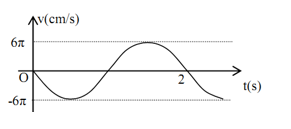
\includegraphics[scale=1]{../figs/VN12-PH-02-A-001-2-V2-2.png}
		\end{center}
		\begin{mcq}(2)
			\item $v=6\pi\ \text{cm/s}$.
			\item $v=-6\pi\ \text{cm/s}$.
			\item $v=0\ \text{cm/s}$.
			\item $v=6\ \text{cm/s}$.
		\end{mcq}
	}
	{\begin{center}
			\textbf{Hướng dẫn giải}
		\end{center}
		
		Theo ví dụ trên, ta có phương trình vận tốc là
		$$v= 6\pi \cos(\pi t + \pi /2)\ \text{cm/s}$$
		
		Ở thời điểm ban đầu ($t=0$) thì $v=6\pi \cos (0+\pi /2) = 0$
		
		\manatip{Nhìn vào đồ thị, ta thấy khi $t=0$ thì $v=0$.}
		
		\textbf{Đáp án: C.}
	}
\end{dang}